\documentclass[conference]{IEEEtran}
\usepackage{cite}
\usepackage{amsmath,amssymb,amsfonts}
\usepackage{algorithmic}
\usepackage{graphicx}
\usepackage{textcomp}
\usepackage{xcolor}
\usepackage[portuguese]{babel}
\usepackage{textgreek}
\selectlanguage{portuguese}
\def\BibTeX{
    {\rm B\kern-.05em{\sc i\kern-.025em b}\kern-.08em T\kern-.1667em\lower.7ex\hbox{E}\kern-.125emX}
}
\fboxsep=0pt
\fboxrule=1pt

\begin{document}

%%%%%%%%%%%%%%%%%%%%%%%%%%%%%%%%%%%%%%%%%%%%%%%%%%%%%%%%%%%%%%%%%%%%%%%%%%%%%%%%
%%%%%%%%%%%%%%%%%%%%%%%%%%%%%%%%%%%%%%%%%%%%%%%%%%%%%%%%%%%%%%%%%%%%%%%%%%%%%%%%
%%%%%%%%%%%%%%%%%%%%%%%%%%%%%%%%%%%%%%%%%%%%%%%%%%%%%%%%%%%%%%%%%%%%%%%%%%%%%%%%

\title{Relatório do Trabalho 1 de Introdução ao Processamento de Imagens\\}

\author{
    \IEEEauthorblockN{Pedro Nogueira}
    \IEEEauthorblockA{
        \textit{Departamento de Ciência da Computação} \\
        \textit{Universidade de Brasília}\\
        Brasília, Brasil \\
        cmcg89034@gmail.com
    }
}

\maketitle

%%%%%%%%%%%%%%%%%%%%%%%%%%%%%%%%%%%%%%%%%%%%%%%%%%%%%%%%%%%%%%%%%%%%%%%%%%%%%%%%
%%%%%%%%%%%%%%%%%%%%%%%%%%%%%%%%%%%%%%%%%%%%%%%%%%%%%%%%%%%%%%%%%%%%%%%%%%%%%%%%
%%%%%%%%%%%%%%%%%%%%%%%%%%%%%%%%%%%%%%%%%%%%%%%%%%%%%%%%%%%%%%%%%%%%%%%%%%%%%%%%

\begin{abstract}
A matéria Introdução a Processamento de Imagens, ministrada na Univesidade de Brasília, pelo professor Bruno Macchiavello, tem por objetivo ensinar a seus alunos diversas operações que são possíveis fazer em imagens. O objetivo da matéria é de formar alunos capazes de aplicar essas operações para diversos fins, desde apagar ruídos de imagens até reconhecimentos sofisticados em suas características visuais. O objetivo desse primeiro projeto é avaliar o entendimento dos estudantes nesse primeiro momento de avaliações da matéria.
\end{abstract}

\begin{IEEEkeywords}
MATLAB, Imagens YUV/RGB, Suavização de píxels por vizinhança, Filtros de convolução, Filtros laplaciano e gaussiano, Imagens no domínio da frequência, Filtros de passa-altas/passa-baixas no domínio da frequência, Filtros rejeita-notch.
\end{IEEEkeywords}

%%%%%%%%%%%%%%%%%%%%%%%%%%%%%%%%%%%%%%%%%%%%%%%%%%%%%%%%%%%%%%%%%%%%%%%%%%%%%%%%
%%%%%%%%%%%%%%%%%%%%%%%%%%%%%%%%%%%%%%%%%%%%%%%%%%%%%%%%%%%%%%%%%%%%%%%%%%%%%%%%
%%%%%%%%%%%%%%%%%%%%%%%%%%%%%%%%%%%%%%%%%%%%%%%%%%%%%%%%%%%%%%%%%%%%%%%%%%%%%%%%

\section{Introdução}

A disciplina começa apresentando processamentos de baixo nível em imagens, que são processamentos que recebem uma imagem como entrada e retornam a própria imagem com algumas modificações. Este primeiro trabalho cobre parte dos conteúdos passados nesse primeiro momento, que são:

\begin{itemize}
    \item Alargamento e suavização de imagens por vizinhança de píxels;
    \item Aplicação de filtros laplacianos e gaussianos;
    \item Desenvolvimento de filtros rejeita-notch.
\end{itemize}

A primeira parte do projeto traz os conceitos de vídeo quadro por quadro, formato de cores YUV, e alargamento e suavização. Um vídeo disposto quadro por quadro é simplesmente uma sequência de bytes que contém cada um dos quadros do vídeo, sendo cada um desses quadros uma imagem correspondente àquele momento do vídeo. O formato de cores YUV, diferente do RGB (\textbf{R}ed \textbf{G}reen \textbf{B}lue), tem por sua composição três imagens, uma contendo o brilho e as outras duas a composição geral das cores da imagem original.

A segunda parte do projeto contém os conceitos de filtros e convoluções no domínio do espaço. Ao se tratar uma imagem como um sinal no domínio do espaço, de coordenadas bidimensionais horizontal e vertical, pode ser feita uma convolução na imagem usando o núcleo desejado, bastando inverter esse núcleo e passá-lo por cada píxel da imagem pra se fazer a média de suas intercessões em cada posição. Os filtros laplaciano e gaussiano são simplesmente filtros que foram elaborados em sua teoria pelos matemáticos Pierre-Simon Laplace e Carl Friedrich Gauss respectivamente.

A terceira parte do trabalho usa os conceitos de imagens no domínio da frequência, filtro passa-altas, filtro Butterworth, e filtros rejeita-notch. Tratando uma imagem como um sinal e aplicando a transformada de Fourier discreta e não-periódica nela, vinda da série calculada pelo matemático Jean-Baptiste Joseph Fourier, obtém-se assim a imagem no domínio da frequência. Essa imagem contém informações das frequências da imagem original, sendo as baixas frequências representativas do formato geral da imagem e as altas frequências representativas das bordas da imagem. Um filtro passa-altas nada mais significa que a aplicação de uma máscara binária ou gradiente que anula baixas frequências da imagem. O filtro Butterworth utilizado no projeto é um filtro calculado pelo engenheiro Stephen Butterworth, e um filtro rejeita-notch é o conjunto de vários filtros passa-altas com seus centros em posições desejadas. Um filtro rejeita-notch é muito útil para a eliminação do efeito de padrões Moiré de uma imagem, o que será executado nesse projeto.

%%%%%%%%%%%%%%%%%%%%%%%%%%%%%%%%%%%%%%%%%%%%%%%%%%%%%%%%%%%%%%%%%%%%%%%%%%%%%%%%
%%%%%%%%%%%%%%%%%%%%%%%%%%%%%%%%%%%%%%%%%%%%%%%%%%%%%%%%%%%%%%%%%%%%%%%%%%%%%%%%
%%%%%%%%%%%%%%%%%%%%%%%%%%%%%%%%%%%%%%%%%%%%%%%%%%%%%%%%%%%%%%%%%%%%%%%%%%%%%%%%

\section{Metodologia}

%%%%%%%%%%%%%%%%%%%%%%%%%%%%%%%%%%%%%%%%%%%%%%%%%%%%%%%%%%%%%%%%%%%%%%%%%%%%%%%%

\subsection{Imagens YUV e alargamento de píxels}

O arquivo \texttt{foreman.yuv} foi disponibilizado para o teste da primeira parte do projeto, que é composto por vários bytes que representam cada um dos quadros de um vídeo. Esse vídeo tem por resolução 352x288, e suas componentes YUV são disponibilizadas no formato 4:2:0, o que significa que a componente Y está na resolução 352x288, enquanto as componentes U e V estão cada uma na metade da resolução em ambos os eixos, ficando então em resolução 176x144. Considerando b uma quantidade de bytes, w a largura de uma imagem, e h a altura de uma imagem, um quadro Q então contém a quantidade de bytes calculada na equação \ref{eq:q1_m_frameBytes}.

\begin{equation}
    Q_{b} = Y_{h} \times Y_{w} + 2 \times (U_{h} \times U_{w}) + 2 \times (V_{h} \times V_{w}) \label{eq:q1_m_frameBytes}
\end{equation}

Para se obter um quadro N (começando em zero) no arquivo, foi preciso primeiro calcular quantos bytes seriam ignorados para então começar a leitura, e isso é equivalente à quantidade de bytes de N quadros.

\begin{equation}
    Q_{inicio} = N \times Q_{b} \label{eq:q1_m_frameStart}
\end{equation}

Como as componentes da imagem estão em dimensões diferentes, foi preciso dobrar a altura e largura das componentes U e V. O professor propôs dois métodos de alargamento: o de replicar cada píxel em um quadrado de 4 píxels 2x2, e o de preencher os píxels novos criados com as médias dos píxels vizinhos, se disponíveis. Um exemplo de um conjunto de seis píxels 3x2 se encontra na tabela \ref{tab:q1_m_original}, e seus dois tipos de alargamento diferentes nas tabelas \ref{tab:q1_m_replicated} e \ref{tab:q1_m_average}.

\begin{table}
    \caption{Píxels originais}
    \centering
    \begin{tabular}{|c|c|c|}
        \hline
        2 & 4 & 6 \\
        \hline
        8 & 10 & 12 \\
        \hline
    \end{tabular}
    \label{tab:q1_m_original}
\end{table}

\begin{table}
    \caption{Píxels replicados}
    \centering
    \begin{tabular}{|c|c|c|c|c|c|}
        \hline
        2 & 2 & 4 & 4 & 6 & 6 \\
        \hline
        2 & 2 & 4 & 4 & 6 & 6 \\
        \hline
        8 & 8 & 10 & 10 & 12 & 12 \\
        \hline
        8 & 8 & 10 & 10 & 12 & 12 \\
        \hline
    \end{tabular}
    \label{tab:q1_m_replicated}
\end{table}

\begin{table}
    \caption{Píxels em média}
    \centering
    \begin{tabular}{|c|c|c|c|c|c|}
        \hline
        2 & 3 & 4 & 5 & 6 & 6 \\
        \hline
        5 & 6 & 7 & 8 & 9 & 6 \\
        \hline
        8 & 9 & 10 & 11 & 12 & 12 \\
        \hline
        8 & 8 & 10 & 10 & 12 & 12 \\
        \hline
    \end{tabular}
    \label{tab:q1_m_average}
\end{table}

Dobradas as dimensões dos componentes U e V, pode-se gerar a imagem RGB ao se usar a função \texttt{ycbcr2rgb()} do MATLAB.

Para dobrar o tamanho total da imagem, foram aplicados os algoritmos de alargamento no componente Y original e nos componentes U e V previamente alargados. Feito isso, as componentes novamente estão em dimensões iguais, sendo possível então usar a função \texttt{ycbcr2rgb()} novamente.

%%%%%%%%%%%%%%%%%%%%%%%%%%%%%%%%%%%%%%%%%%%%%%%%%%%%%%%%%%%%%%%%%%%%%%%%%%%%%%%%

\subsection{Filtros de convolução no domínio do espaço}

A segunda parte do projeto prevê que o aluno deve fazer filtragens por convolução na imagem \texttt{Image1.pgm} no domínio do espaço, ou seja, na própria imagem. A convolução das imagens foram todas feitas usando núcleos específicos com a função \texttt{imfilter()}. Foram usados quatro núcleos diferentes para essas filtragens: dois foram obtidos com a função do MATLAB \texttt{fspecial()} com os parâmetros \texttt{'gaussian'} para o modo do núcleo e 3 para a dimensão do núcleo, mudando somente o terceiro parâmetro \textsigma\ para 0.5 ou para 1 quando requisitado; e dois desses núcleos são os laplacianos de tamanho 3x3 e centro -4 e -8 representados nas tabelas \ref{tab:q2_m_laplace4} e \ref{tab:q2_m_laplace8} respectivamente.

\begin{table}
    \centering
    \begin{minipage}{.49\linewidth}
        \caption{LaPlaciano centro -4}
        \centering
        \begin{tabular}{|c|c|c|}
            \hline
            0 & 1 & 0 \\
            \hline
            1 & -4 & 1 \\
            \hline
            0 & 1 & 0 \\
            \hline
        \end{tabular}
        \label{tab:q2_m_laplace4}
    \end{minipage}
    \begin{minipage}{.49\linewidth}
        \caption{LaPlaciano centro -8}
        \centering
        \begin{tabular}{|c|c|c|}
            \hline
            1 & 1 & 1 \\
            \hline
            1 & -8 & 1 \\
            \hline
            1 & 1 & 1 \\
            \hline
        \end{tabular}
        \label{tab:q2_m_laplace8}
    \end{minipage}
\end{table}

\begin{figure}
    \centering
    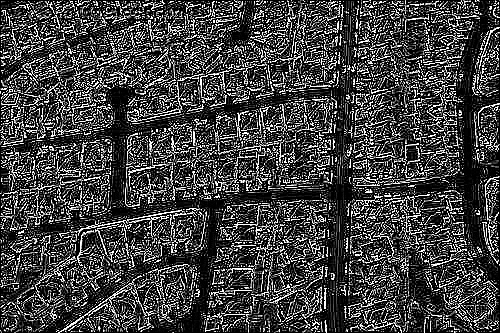
\includegraphics[width=0.37\textwidth]{imgs/Q2-2 LaPlace filtered (k 3x3 c-8).png}
    \caption\scriptsize{Resultado da aplicação do filtro laplaciano em \texttt{Image1.pgm}}
    \label{fig:q2_m_laplaceFilter3x3c8}
\end{figure}

A aplicação do filtro gaussiano suaviza a imagem. O filtro laplaciano cria uma imagem com as bordas e contornos da original, que é usada para subtrair da imagem original e obter uma imagem com os contornos destacados. A figura \ref{fig:q2_m_laplaceFilter3x3c8} é exemplo de uma imagem obtida pela aplicação direta do filtro laplaciano 3x3 com centro -8. Então, três procedimentos foram executados:

Primeiro foi pedido que se fizesse a convolução com o filtro laplaciano de centro -8 diretamente.

Depois foi pedido que fosse aplicado primeiramente um filtro gaussiano de \textsigma\ = 0.5 para depois aplicar um filtro laplaciano de centro -4.

Por último, foi aplicado um filtro gaussiano de \textsigma\ = 1 para depois aplicar um filtro laplaciano de centro -4.

%%%%%%%%%%%%%%%%%%%%%%%%%%%%%%%%%%%%%%%%%%%%%%%%%%%%%%%%%%%%%%%%%%%%%%%%%%%%%%%%

\subsection{Filtragem rejeita-notch no domínio da frequência}

Na terceira e última parte do projeto foi requisitado que fosse feita uma filtragem rejeita-notch de frequências especificadas pelas instruções do projeto na imagem \texttt{moire.tif}, que tem padrões de Moiré extremamente evidentes pela imagem toda.

Para isso, foi primeiramente necessário transformar a imagem para o domínio da frequência usando a função do MATLAB \texttt{fft2()} e reposicionar os quadrantes da imagem de forma que as baixas frequências fiquem no centro da imagem e as altas nos cantos e bordas usando a função \texttt{fftshift()}.

\begin{figure}
    \centering
    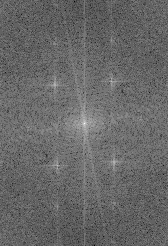
\includegraphics[]{imgs/Q3-2 Reject Notch original Fourier.png}
    \caption\scriptsize{Imagem \texttt{moire.tif} no domínio da frequência com os quadrantes reposicionados}
    \label{fig:q3_m_frequencyOriginal}
\end{figure}

O filtro rejeita-notch requisitado pelas especificações foi o filtro Butterworth, filtro passa-altas que gradualmente vai de zero a um conforme a distância D(k,l) do centro do filtro até um raio D\texorpdfstring{\textsubscript{0}}\\ com um expoente n. A equação do gradiente Butterworth é dada na equação \ref{eq:q3_m_butterworth}.

\begin{equation}
    H(k,l) = \sqrt{\frac{1}{1 + (\frac{D_{0}}{D(k,l)})^{2n}}} \label{eq:q3_m_butterworth}
\end{equation}

O projeto especificou as posições relativas ao centro da imagem transformada e os raios dos filtros de Butterworth a serem aplicados nessas posições, e esses dados são:

\begin{itemize}
    \item D\texorpdfstring{\textsubscript{0}}\\ = 10, u\texorpdfstring{\textsubscript{k}}\\ = 39, v\texorpdfstring{\textsubscript{k}}\\ = 30
    \item D\texorpdfstring{\textsubscript{0}}\\ = 10, u\texorpdfstring{\textsubscript{k}}\\ = -39, v\texorpdfstring{\textsubscript{k}}\\ = 30
    \item D\texorpdfstring{\textsubscript{0}}\\ = 5, u\texorpdfstring{\textsubscript{k}}\\ = 78, v\texorpdfstring{\textsubscript{k}}\\ = 30
    \item D\texorpdfstring{\textsubscript{0}}\\ = 5, u\texorpdfstring{\textsubscript{k}}\\ = -78, v\texorpdfstring{\textsubscript{k}}\\ = 30
\end{itemize}

Essas posições u\texorpdfstring{\textsubscript{k}}\\ e v\texorpdfstring{\textsubscript{k}}\\ relativas ao centro são os locais onde se deve aplicar os filtros rejeita-notch. Entretanto, por definição, uma imagem no domínio da frequência carrega a mesma frequência em dois pontos, onde ambos são opostos verticalmente e horizontalmente, o que significa que esse filtro Butterworth precisa ser aplicado em oito posições. Foi criada então uma máscara contendo esses filtros de Butterworth, representada pela figura \ref{fig:q3_m_butterworth}, para que essa fosse aplicada de uma só vez na imagem no domínio da frequência.

\begin{figure}
    \centering
    \fbox{
        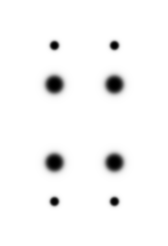
\includegraphics[]{imgs/Q3-3 Reject Notch mask.png}
    }
    \caption\scriptsize{Máscara contendo os filtros de Butterworth}
    \label{fig:q3_m_butterworth}
\end{figure}

A aplicação de filtros deve ser feita por convolução no domínio do espaço, mas há uma facilidade no domínio da frequência para essa aplicação, pois ela se resume à simples multiplicação da máscara e da transformada. Feita a filtragem, basta fazer o reposicionamento dos quadrantes da imagem de volta pra as posições iniciais com \texttt{fftshift()} e aplicar a transformada de Fourier novamente com \texttt{fft2()}.

%%%%%%%%%%%%%%%%%%%%%%%%%%%%%%%%%%%%%%%%%%%%%%%%%%%%%%%%%%%%%%%%%%%%%%%%%%%%%%%%
%%%%%%%%%%%%%%%%%%%%%%%%%%%%%%%%%%%%%%%%%%%%%%%%%%%%%%%%%%%%%%%%%%%%%%%%%%%%%%%%
%%%%%%%%%%%%%%%%%%%%%%%%%%%%%%%%%%%%%%%%%%%%%%%%%%%%%%%%%%%%%%%%%%%%%%%%%%%%%%%%

\section{Resultados}

%%%%%%%%%%%%%%%%%%%%%%%%%%%%%%%%%%%%%%%%%%%%%%%%%%%%%%%%%%%%%%%%%%%%%%%%%%%%%%%%

\subsection{Imagens YUV e alargamento de píxels}

Duas imagens finais foram geradas, uma com alargamento por replicação de píxels (figura \ref{fig:q1_r_replication}) e outra por média de píxels vizinhos (figura \ref{fig:q1_r_average}).

\begin{figure}
    \centering
    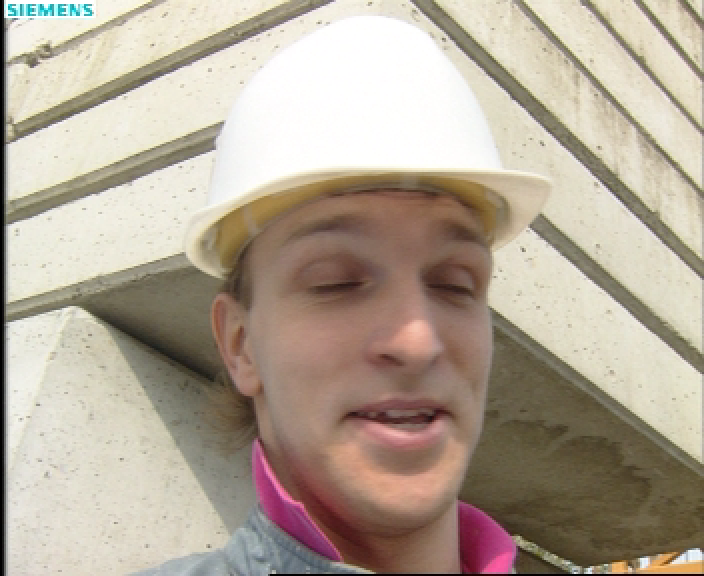
\includegraphics[width=0.33\textwidth]{imgs/Q1-3 YUV to RGB large.png}
    \caption\scriptsize{Imagem YUV alargada por replicação}
    \label{fig:q1_r_replication}
\end{figure}

\begin{figure}
    \centering
    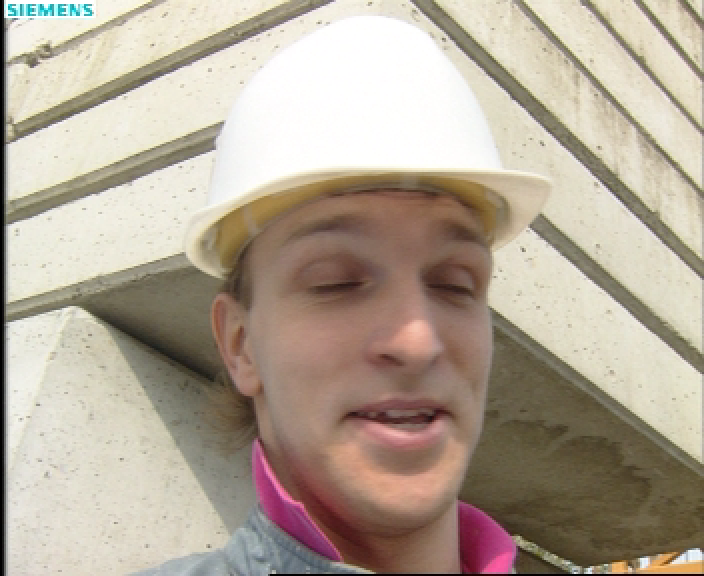
\includegraphics[width=0.35\textwidth]{imgs/Q1-3 YUV to RGB large.png}
    \caption\scriptsize{Imagem YUV alargada por cálculo de média}
    \label{fig:q1_r_average}
\end{figure}

Após tanto alargar os componentes U e V responsáveis pelas cores da imagem, esperava-se que algum defeito ficasse mais aparente, mas o que mais interferiu na imagem foi a modificação na componente de brilho Y. O método de alargamento de píxel por cálculo de média dos vizinhos é subjetivamente melhor que o método de simples replicação dos píxels, o que é aparente principalmente no texto no canto superior da esquerda "SIEMENS".

%%%%%%%%%%%%%%%%%%%%%%%%%%%%%%%%%%%%%%%%%%%%%%%%%%%%%%%%%%%%%%%%%%%%%%%%%%%%%%%%

\subsection{Filtros de convolução no domínio do espaço}

Os três procedimentos diferentes geraram as três imagens representadas pelas figuras \ref{fig:q2_r_laplace-8}, \ref{fig:q2_r_gaussHalf} e \ref{fig:q2_r_gauss1}.

\begin{figure}
    \centering
    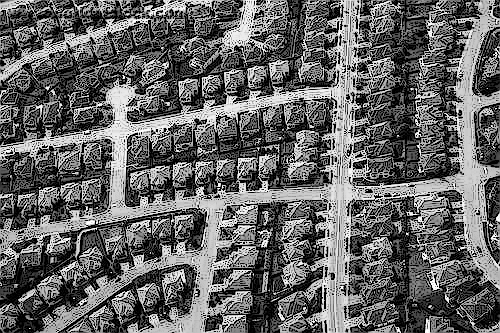
\includegraphics[width=0.37\textwidth]{imgs/Q2-3 LaPlace added (k 3x3 c-8).png}
    \caption\scriptsize{Imagem com aplicação do filtro laplaciano 3x3 de centro -8}
    \label{fig:q2_r_laplace-8}
\end{figure}

\begin{figure}
    \centering
    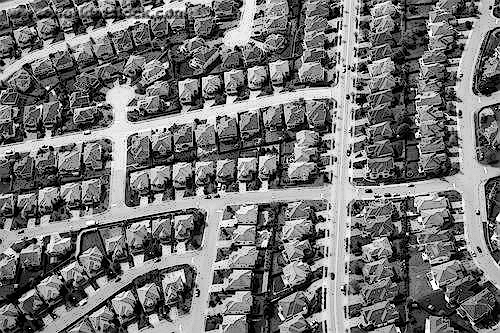
\includegraphics[width=0.37\textwidth]{imgs/Q2-5 Gauss LaPlace added (3x3 sigma 0.5 k 3x3 c-4).png}
    \caption\scriptsize{Imagem com aplicação do filtro gaussiano de \textsigma\ 0.5 e laplaciano 3x3 de centro -4}
    \label{fig:q2_r_gaussHalf}
\end{figure}

\begin{figure}
    \centering
    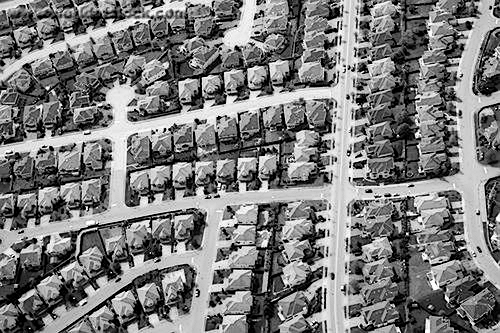
\includegraphics[width=0.37\textwidth]{imgs/Q2-7 Gauss LaPlace added (3x3 sigma 1 k 3x3 c-4).png}
    \caption\scriptsize{Imagem com aplicação do filtro gaussiano de \textsigma\ 1 e laplaciano 3x3 de centro -4}
    \label{fig:q2_r_gauss1}
\end{figure}

O primeiro procedimento, por ter sido somente uma filtragem passa-altas, foi muito abrupto em sua execução, deixando a imagem com as bordas muito acentuadas. Os próximos procedimentos fizeram uma filtragem passa-altas também, mas só depois de fazer uma suavização da imagem, tornando-a mais coerente para visualização.

%%%%%%%%%%%%%%%%%%%%%%%%%%%%%%%%%%%%%%%%%%%%%%%%%%%%%%%%%%%%%%%%%%%%%%%%%%%%%%%%

\subsection{Filtragem rejeita-notch no domínio da frequência}

Inicialmente, \texttt{moire.tiff}, a imagem usada nessa parte do projeto, continha padrões de Moiré muito proeminentes na forma de diversos "quadradinhos" pela imagem, e como indicado no resultado do procedimento (figura \ref{fig:q3_r_car}), esse padrão desapareceu da maioria da imagem. Mais próximo das bordas ainda há o efeito Moiré, e isso se dá por não ter sido feito padding na imagem no domínio da frequência antes de fazer sua filtragem rejeita-notch.

\begin{figure}
    \centering
    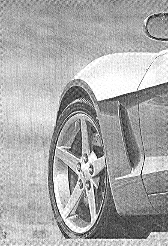
\includegraphics[]{imgs/Q3-4 Reject Notch result.png}
    \caption\scriptsize{Imagem \texttt{moire.tiff} após aplicação do filtro rejeita-notch}
    \label{fig:q3_r_car}
\end{figure}

%%%%%%%%%%%%%%%%%%%%%%%%%%%%%%%%%%%%%%%%%%%%%%%%%%%%%%%%%%%%%%%%%%%%%%%%%%%%%%%%
%%%%%%%%%%%%%%%%%%%%%%%%%%%%%%%%%%%%%%%%%%%%%%%%%%%%%%%%%%%%%%%%%%%%%%%%%%%%%%%%
%%%%%%%%%%%%%%%%%%%%%%%%%%%%%%%%%%%%%%%%%%%%%%%%%%%%%%%%%%%%%%%%%%%%%%%%%%%%%%%%

\section{Conclusões}

Todos os procedimentos desse primeiro trabalho foram realizados com sucesso. Os resultados dos procedimentos foram esperados por terem sido assunto das aulas de Introdução ao Processamento de Imagens, mas ainda assim foi surpreendente testemunhar a gama de possibilidades em que uma imagem pode ser processada. O projeto foi um sucesso em sua execução como um todo, portanto as aulas também foram um sucesso no ensinamento de seus dicentes.

%%%%%%%%%%%%%%%%%%%%%%%%%%%%%%%%%%%%%%%%%%%%%%%%%%%%%%%%%%%%%%%%%%%%%%%%%%%%%%%%
%%%%%%%%%%%%%%%%%%%%%%%%%%%%%%%%%%%%%%%%%%%%%%%%%%%%%%%%%%%%%%%%%%%%%%%%%%%%%%%%
%%%%%%%%%%%%%%%%%%%%%%%%%%%%%%%%%%%%%%%%%%%%%%%%%%%%%%%%%%%%%%%%%%%%%%%%%%%%%%%%

\begin{thebibliography}{00}
    \bibitem{b1} Slides das aulas de Introdução ao Processamento de Imagens do professor Bruno Macchiavello, Universidade de Brasília.
\end{thebibliography}

\end{document}
